\documentclass[titlepage]{article}
\usepackage[utf8]{inputenc}
\usepackage{amsmath}
\usepackage{algpseudocode}
\usepackage[]{graphicx}
\usepackage{hyperref}
\usepackage[margin=0.8in]{geometry}
\title{Special multiplication of two digit numbers}
\author{Siddharth Mittal}
\date{$6^{th}$ March 2017}

\begin{document}
\maketitle

%Section1
\section{Introduction}
\label{sec:intro}
The aim of this document is to explain to the reader a fast way to multiply two, two digit numbers, given that they meet certain criteria.
\\
\\
We'll be going over the algorithm \cite{atharv} and also the correctness of the algorithm \cite{sidpaper}.

%Section2
\section{Example}
\label{sec:example}
Let us first look at examples \footnote{Pretty Amazing, Eh?} , to understand what is happening.
\subsection{Case 1}
\label{subsec:c1}
The first case is when the first(tens') digits are same and the last ones add to ten.
If we take the numbers to be as $10x+y$ and $10x+z$ and $y+z=10$
In such case product becomes\footnote{ $x : y$ means $100x + y$}
$$x(x+1) : yz$$
The figure given below will clear the scheme of things:
\begin{figure}[h]
\centering
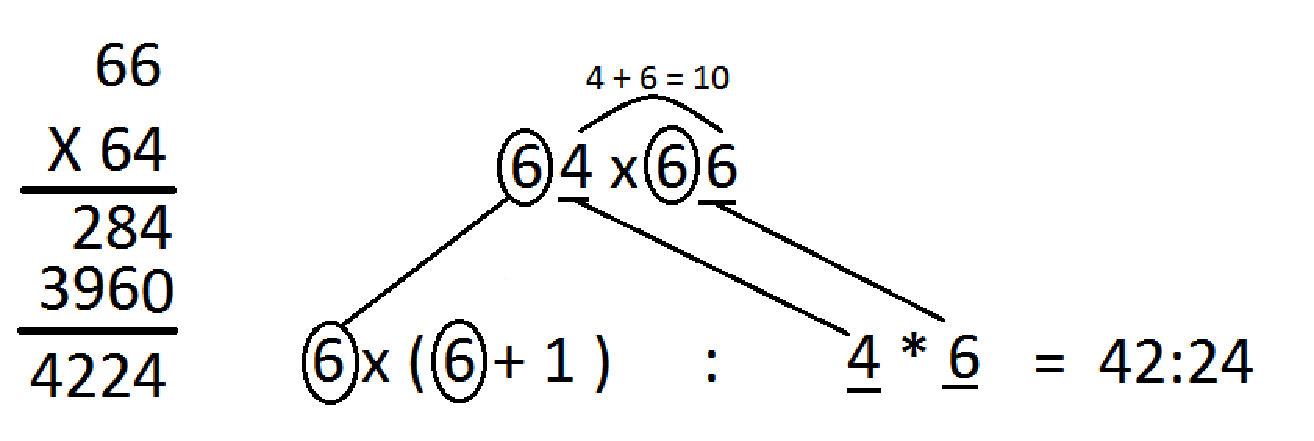
\includegraphics[scale=0.4]{case1.pdf}
\end{figure}
\subsection{Case 2}
\label{subsec:c2}
The second case is when the first digits add to ten and the last ones are same.
If we take the numbers to be as $10x+y$ and $10z+y$ and $x+z=10$
In such case product becomes
$$xz + y : y^2$$
The figure given below will clear the scheme of things:
\begin{figure}[h]
\centering
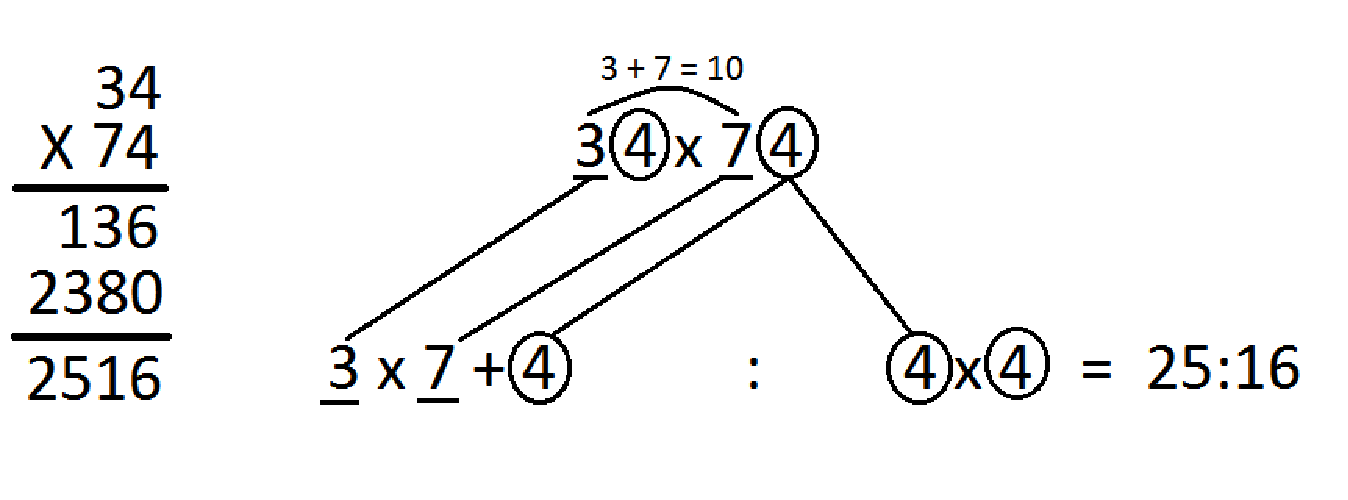
\includegraphics[scale=0.4]{case2.pdf}
\end{figure}
\newpage
\section{Why this Rocks}
The above method is simply amazing because we have to spend very less time and effort in calculating the product of two 2-digit numbers, given that they satisfy one of the criteria.
This is very clear from the examples given in the Section \ref{sec:example}.
%Section3: Highlighting the proof of algorithm
\section{Proof of Correctness}
\label{sec:proof}
\subsection{Case 1}
We highlight the proof for Case 1.
\\
Say we have two numbers, one is $xy$ and the other is $xz$ such that $y+z=10$. Therefore the result of multiplication of these numbers, say $a$, is going to be:
\begin{align*}
a &= (10x+y)*(10x+z) \\
 &= 100x^2+10xz+10xy+yz \\
 &= 100x^2+10xy+10x(10-y)+y(10-y)\\
 &= 100x^2+10xy+100x-10xy+10y-y^2\\
 &= 100x^2+100x+10y-y^2\\
a &= 100x(x+1)+yz
\end{align*}
This is precisely what the algorithm gives. It says take the first part as $x(x+1)$ and take the second part as $yz$. That is, the product is $x(x+1):yz$.
\subsection{Case 2}
Now, the proof for Case 2.\\
Let the two numbers be such that one is $xy$ and the other is $zy$. Let the product of these numbers be $a$. Then,
\begin{align*}
a &= (10x+y)(10z+y) \\ 
&=100xz+10xy+10zy+y^2\\
&=100xz+10y(x+z)+y^2\\
&=100xz+10y(10)+y^2 \hspace{50} [\text{Substituting } x+z=10]\\
&=100xz+100y+y^2\\
&=100(xz+y)+y^2
\end{align*}
This is exactly what the algorithm tells us to do. It says take the first part as $xz+y$ and take the second part as $y^2$. That is, the product is $xz+y:y^2$.
\newpage
\section{Pseudocode}
$n1$ and $n2$ are the two 2-digit numbers that we are going to multiply.
\begin{algorithmic}
    \State \textbf{int Multiply2}(int n1,int n2)\{
     \State$x_1 \leftarrow n1/10;$  
     \State$y_1 \leftarrow n1\%10;$
     \State$x_2 \leftarrow n2/10;$
     \State$y_2 \leftarrow n2\%10;$
     \State \If{$x_1 == x_2, y_1 + y_2==10 $}
         \Comment{Case1}
         \State$f1\leftarrow x_1*(x_1+1);$  
         \State$f2\leftarrow y_1*y_2;$  
         \State$prod\leftarrow 100*f1+f2;$
     \EndIf
     \State \If{$x_1+x_2==10,y_1==y_2$}
        \Comment{Case2}
        \State$f1\leftarrow x_1*x_2+y_1;$
        \State$f2\leftarrow {y_1}^2;$
        \State$prod\leftarrow 100*f1+f2;$
     \EndIf
\\
\}
\end{algorithmic}

\section{Generalization}
We can generalize this. Let us look at how to do it. The arithmetic proofs remain similar to the 2-digit case. We consider two r-digit numbers.
\begin{table}[h]
\begin{center}
\begin{tabular}{|c|c|c|c|}
    \hline
    Case & What is same & What adds to what & Product\\
    \hline
    Case1 & The first digit & Last $r-1$ add to $10^{r-1}$ & $10^{2r-2}x(x+1)+y_1*y_2$\\
    \hline
    Case2 & The last digit & First $r-1$ add to $10^{r-1}$ & $10^{2r-2}(y_1*y_2+x)+x^2$\\
    \hline
    Case3 & First r digits & Last digits add to 10 & $10^{2r-2}x(x + 1)+yz$\\
    \hline
    Case4 & Last r digits & First digits add to 10 & $10^{2r-2}(xz+y)+y^2$\\
    \hline
\end{tabular}
\end{center}
\end{table}
\subsection{Case 1}
Let the first digit(the one at $r_{th}$ place) be x. Let the two remaining parts be $y_1$ and $y_2$. Then the product is $10^{2r-2}x(x+1)+y_1*y_2$
\subsection{Case 2}
Let the last digit(the one at ones' place) be x. Let the two remaining parts be $y_1$ and $y_2$. Then the product is $10^{2r-2}(y_1*y_2+x)+x^2$
\subsection{Case 3}
Let the first $r-1$ digits be x. The last digits of two numbers be $y$ and $z$. Then the product is $10^{2r-2}x(x + 1)+yz$
\subsection{Case 4}
Let the last $r-1$ digits be y. The first digits of two numbers be $x$ and $z$. Then the product is $10^{2r-2}(xz+y)+y^2$
\newpage
%Section for timepass
\section{Miscellaneous}
\label{sec:misc}
You can find an amazing tool to visualize and understand this kind of fast multiplication at my site\footnote{Just Kidding.} : \url{home.iitk.ac.in/~sidm/}
%Bibliography options
\bibliographystyle{unsrt}
\bibliography{biblio}
\end{document}
